

\begin{figure}[tb]

{\centering 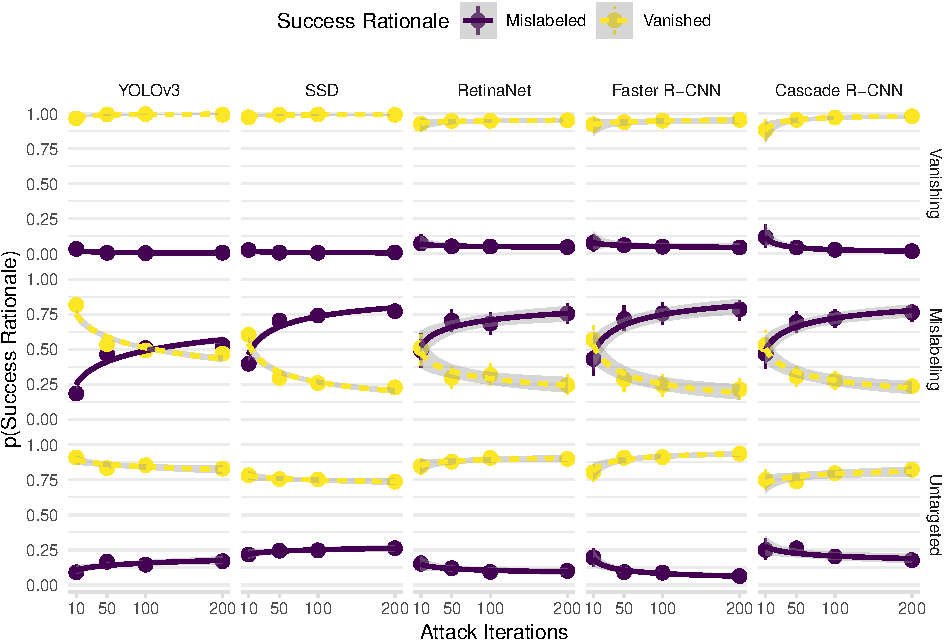
\includegraphics{rmd_imgs/success_trend_breakdown_graph-1} 

}

\caption{\textbf{Vanishing and mislabeling attacks mostly cause target objects to vanish and get mislabeled:}  The graph breaks down the success rationale within the success cases (Figure \ref{fig:success_trend_graph}). Though we did not restrict success to the intended attack mode (e.g. a vanishing attack which mislabels the target object still count as a success case), the target objects do vanish and get mislabeled in most success cases respectively in the vanishing and mislabeling attacks. The binned summaries and regression trendlines break down the success cases into proportion vanished and mislabeled---separated by attack---against attack iterations in the randomized attack experiment. Errors are 95\% confidence intervals. }\label{fig:success_trend_breakdown_graph}
\end{figure}

\begin{figure}[tb]

{\centering 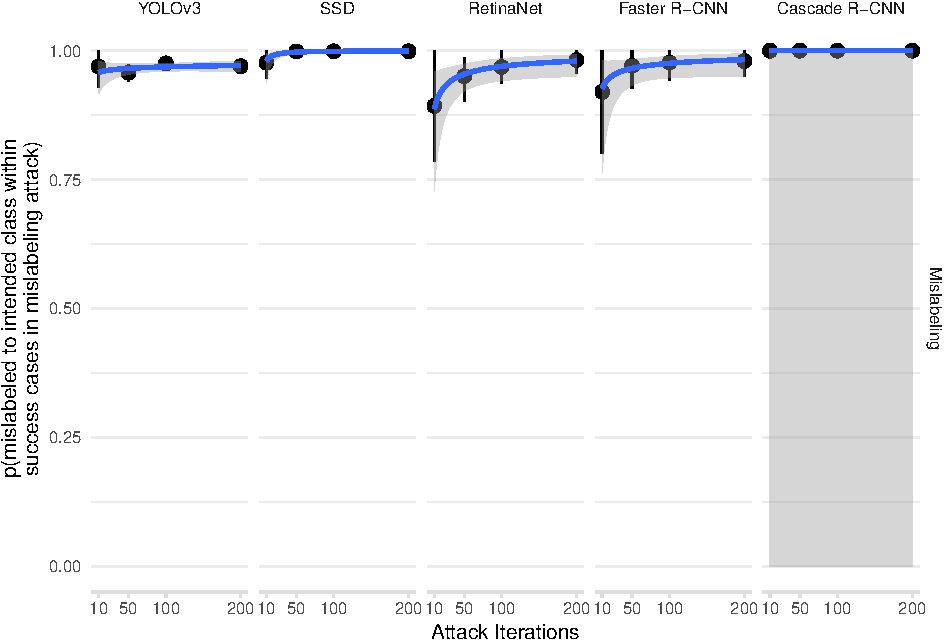
\includegraphics{rmd_imgs/success_trend_mislabel_intended_graph-1} 

}

\caption{\textbf{Mislabeling attacks usually mislabel the target objects to the intended class:}  The binned summaries and regression trendlines give us the proportion mislabeled to the intended class within the success cases in the mislabeling attack. The proportion is plotted against attack iterations in the randomized attack experiment. Errors are 95\% confidence intervals.  For Cascade R-CNN, the logistic model did not converge because the mislabel intended proportion is constant at 100\%.}\label{fig:success_trend_mislabel_intended_graph}
\end{figure}

\begingroup\fontsize{9}{11}\selectfont

\begin{longtable}[t]{lllrrrrrr}
\caption{\label{tab:model_stage_table}We run a logistic model regressing success against detection models, split by attack, in the randomized attack experiment. All attacks, especially vanishing and mislabeling, obtain higher success on 1-stage (YOLOv3, SSD) than 2-stage (Faster R-CNN, Cascade R-CNN) detectors. However, the 1-stage RetinaNet is as resilient as 2-stage detectors. Table headers are explained in Appendix \ref{app:tab_hdr}.}\\
\toprule
\multicolumn{1}{c}{Group} & \multicolumn{8}{c}{Regression} \\
\cmidrule(l{3pt}r{3pt}){1-1} \cmidrule(l{3pt}r{3pt}){2-9}
Attack & term & sig & estimate & std.error & statistic & p.value & conf.low & conf.high\\
\midrule
 & YOLOv3 &  & 0.000 &  &  &  &  & \\
\cmidrule{2-9}\nopagebreak
 & SSD &  & 0.041 & 0.044 & 0.924 & 0.355 & -0.046 & 0.127\\
\cmidrule{2-9}\nopagebreak
 & RetinaNet & * & -1.492 & 0.060 & -24.865 & 0.000 & -1.610 & -1.375\\
\cmidrule{2-9}\nopagebreak
 & Faster R-CNN & * & -2.161 & 0.075 & -28.651 & 0.000 & -2.311 & -2.015\\
\cmidrule{2-9}\nopagebreak
\multirow{-5}{*}{\raggedright\arraybackslash Vanishing} & Cascade R-CNN & * & -1.788 & 0.066 & -27.097 & 0.000 & -1.919 & -1.660\\
\cmidrule{1-9}\pagebreak[0]
 & YOLOv3 &  & 0.000 &  &  &  &  & \\
\cmidrule{2-9}\nopagebreak
 & SSD & * & -0.283 & 0.046 & -6.183 & 0.000 & -0.372 & -0.193\\
\cmidrule{2-9}\nopagebreak
 & RetinaNet & * & -2.594 & 0.089 & -29.029 & 0.000 & -2.773 & -2.422\\
\cmidrule{2-9}\nopagebreak
 & Faster R-CNN & * & -2.752 & 0.095 & -28.826 & 0.000 & -2.944 & -2.569\\
\cmidrule{2-9}\nopagebreak
\multirow{-5}{*}{\raggedright\arraybackslash Mislabeling} & Cascade R-CNN & * & -2.259 & 0.078 & -28.907 & 0.000 & -2.415 & -2.109\\
\cmidrule{1-9}\pagebreak[0]
 & YOLOv3 &  & 0.000 &  &  &  &  & \\
\cmidrule{2-9}\nopagebreak
 & SSD & * & 0.782 & 0.058 & 13.411 & 0.000 & 0.668 & 0.896\\
\cmidrule{2-9}\nopagebreak
 & RetinaNet & * & -0.239 & 0.069 & -3.463 & 0.001 & -0.375 & -0.104\\
\cmidrule{2-9}\nopagebreak
 & Faster R-CNN &  & -0.031 & 0.066 & -0.462 & 0.644 & -0.160 & 0.099\\
\cmidrule{2-9}\nopagebreak
\multirow{-5}{*}{\raggedright\arraybackslash Untargeted} & Cascade R-CNN & * & -0.505 & 0.074 & -6.850 & 0.000 & -0.650 & -0.361\\
\bottomrule
\end{longtable}
\endgroup{}

\begingroup\fontsize{9}{11}\selectfont

\begin{longtable}[t]{lllrrrrrr}
\caption{\label{tab:target_untarget_vanish_mislabel_table}We run a logistic model regressing success against attacks, split by detection models in the randomized attack experiment. Targeted attacks achieve higher success than untargeted attack on YOLOv3 and SSD. Within targeted attacks, vanishing attacks achieve higher success than mislabeling attack, except on YOLOv3. Table headers are explained in Appendix \ref{app:tab_hdr}.}\\
\toprule
\multicolumn{1}{c}{Group} & \multicolumn{8}{c}{Regression} \\
\cmidrule(l{3pt}r{3pt}){1-1} \cmidrule(l{3pt}r{3pt}){2-9}
Model & term & sig & estimate & std.error & statistic & p.value & conf.low & conf.high\\
\midrule
 & Vanishing &  & 0.000 &  &  &  &  & \\
\cmidrule{2-9}\nopagebreak
 & Mislabeling &  & 0.005 & 0.044 & 0.110 & 0.912 & -0.082 & 0.091\\
\cmidrule{2-9}\nopagebreak
\multirow{-3}{*}{\raggedright\arraybackslash YOLOv3} & Untargeted & * & -1.250 & 0.056 & -22.340 & 0.000 & -1.360 & -1.141\\
\cmidrule{1-9}\pagebreak[0]
 & Vanishing &  & 0.000 &  &  &  &  & \\
\cmidrule{2-9}\nopagebreak
 & Mislabeling & * & -0.318 & 0.046 & -6.990 & 0.000 & -0.408 & -0.229\\
\cmidrule{2-9}\nopagebreak
\multirow{-3}{*}{\raggedright\arraybackslash SSD} & Untargeted & * & -0.509 & 0.047 & -10.844 & 0.000 & -0.601 & -0.417\\
\cmidrule{1-9}\pagebreak[0]
 & Vanishing &  & 0.000 &  &  &  &  & \\
\cmidrule{2-9}\nopagebreak
 & Mislabeling & * & -1.097 & 0.098 & -11.181 & 0.000 & -1.292 & -0.907\\
\cmidrule{2-9}\nopagebreak
\multirow{-3}{*}{\raggedright\arraybackslash RetinaNet} & Untargeted &  & 0.003 & 0.072 & 0.036 & 0.971 & -0.139 & 0.145\\
\cmidrule{1-9}\pagebreak[0]
 & Vanishing &  & 0.000 &  &  &  &  & \\
\cmidrule{2-9}\nopagebreak
 & Mislabeling & * & -0.586 & 0.113 & -5.171 & 0.000 & -0.811 & -0.366\\
\cmidrule{2-9}\nopagebreak
\multirow{-3}{*}{\raggedright\arraybackslash Faster R-CNN} & Untargeted & * & 0.881 & 0.083 & 10.587 & 0.000 & 0.719 & 1.045\\
\cmidrule{1-9}\pagebreak[0]
 & Vanishing &  & 0.000 &  &  &  &  & \\
\cmidrule{2-9}\nopagebreak
 & Mislabeling & * & -0.466 & 0.092 & -5.056 & 0.000 & -0.648 & -0.287\\
\cmidrule{2-9}\nopagebreak
\multirow{-3}{*}{\raggedright\arraybackslash Cascade R-CNN} & Untargeted &  & 0.033 & 0.082 & 0.408 & 0.683 & -0.127 & 0.193\\
\bottomrule
\end{longtable}
\endgroup{}

\begingroup\fontsize{9}{11}\selectfont

\begin{longtable}[t]{llllrrrrrr}
\caption{\label{tab:num_iteration_table}We run a logistic model regressing success against log(attack iterations) in the randomized attack experiment. Success rates increase with attack iterations for all models and attacks. Table headers are explained in Appendix \ref{app:tab_hdr}.}\\
\toprule
\multicolumn{2}{c}{Group} & \multicolumn{8}{c}{Regression} \\
\cmidrule(l{3pt}r{3pt}){1-2} \cmidrule(l{3pt}r{3pt}){3-10}
 & Attack & term & sig & estimate & std.error & statistic & p.value & conf.low & conf.high\\
\midrule
\addlinespace[0.3em]
\multicolumn{10}{l}{\textbf{YOLOv3}}\\
\hspace{1em} & Vanishing & log(iterations) & * & 0.480 & 0.018 & 26.729 & 0 & 0.445 & 0.515\\
\cmidrule{2-10}\nopagebreak
\hspace{1em} & Mislabeling & log(iterations) & * & 0.397 & 0.017 & 23.267 & 0 & 0.363 & 0.430\\
\cmidrule{2-10}\nopagebreak
\hspace{1em} & Untargeted & log(iterations) & * & 0.174 & 0.023 & 7.404 & 0 & 0.128 & 0.220\\
\cmidrule{1-10}\pagebreak[0]
\addlinespace[0.3em]
\multicolumn{10}{l}{\textbf{SSD}}\\
\hspace{1em} & Vanishing & log(iterations) & * & 0.528 & 0.018 & 29.009 & 0 & 0.493 & 0.564\\
\cmidrule{2-10}\nopagebreak
\hspace{1em} & Mislabeling & log(iterations) & * & 0.452 & 0.019 & 23.386 & 0 & 0.414 & 0.490\\
\cmidrule{2-10}\nopagebreak
\hspace{1em} & Untargeted & log(iterations) & * & 0.246 & 0.018 & 13.735 & 0 & 0.211 & 0.281\\
\cmidrule{1-10}\pagebreak[0]
\addlinespace[0.3em]
\multicolumn{10}{l}{\textbf{RetinaNet}}\\
\hspace{1em} & Vanishing & log(iterations) & * & 0.475 & 0.033 & 14.339 & 0 & 0.411 & 0.541\\
\cmidrule{2-10}\nopagebreak
\hspace{1em} & Mislabeling & log(iterations) & * & 0.312 & 0.048 & 6.489 & 0 & 0.219 & 0.408\\
\cmidrule{2-10}\nopagebreak
\hspace{1em} & Untargeted & log(iterations) & * & 0.328 & 0.029 & 11.206 & 0 & 0.271 & 0.385\\
\cmidrule{1-10}\pagebreak[0]
\addlinespace[0.3em]
\multicolumn{10}{l}{\textbf{Faster R-CNN}}\\
\hspace{1em} & Vanishing & log(iterations) & * & 0.394 & 0.042 & 9.316 & 0 & 0.313 & 0.479\\
\cmidrule{2-10}\nopagebreak
\hspace{1em} & Mislabeling & log(iterations) & * & 0.264 & 0.051 & 5.204 & 0 & 0.166 & 0.364\\
\cmidrule{2-10}\nopagebreak
\hspace{1em} & Untargeted & log(iterations) & * & 0.440 & 0.030 & 14.511 & 0 & 0.381 & 0.500\\
\cmidrule{1-10}\pagebreak[0]
\addlinespace[0.3em]
\multicolumn{10}{l}{\textbf{Cascade R-CNN}}\\
\hspace{1em} & Vanishing & log(iterations) & * & 0.495 & 0.039 & 12.772 & 0 & 0.420 & 0.572\\
\cmidrule{2-10}\nopagebreak
\hspace{1em} & Mislabeling & log(iterations) & * & 0.327 & 0.042 & 7.758 & 0 & 0.245 & 0.410\\
\cmidrule{2-10}\nopagebreak
\hspace{1em} & Untargeted & log(iterations) & * & 0.291 & 0.033 & 8.886 & 0 & 0.228 & 0.356\\
\bottomrule
\end{longtable}
\endgroup{}

\begin{figure}[tb]

{\centering 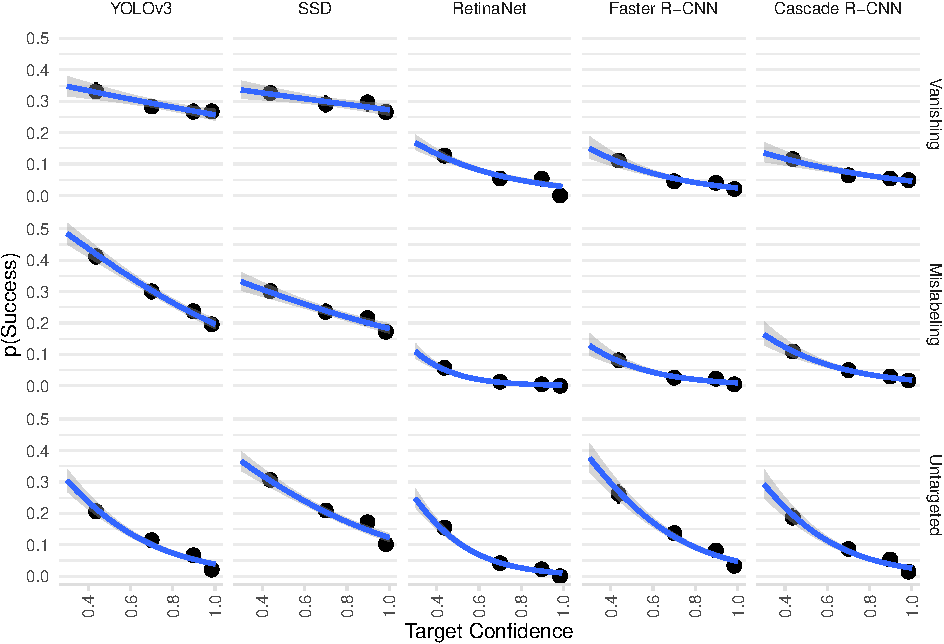
\includegraphics{rmd_imgs/target_conf_graph-1} 

}

\caption{\textbf{Lower target confidence significantly increases success rates for all models and attacks:}  The binned summaries and regression trendlines graph success proportion against target confidence in the randomized attack experiment. Bins are split into quantiles. Errors are 95\% confidence intervals. }\label{fig:target_conf_graph}
\end{figure}

\begingroup\fontsize{9}{11}\selectfont

\begin{longtable}[t]{llllrrrrrr}
\caption{\label{tab:target_conf_table}We run a logistic model regressing success against target confidence in the randomized attack experiment. Lower target confidence significantly increases success rates for all models and attacks. Table headers are explained in Appendix \ref{app:tab_hdr}.}\\
\toprule
\multicolumn{2}{c}{Group} & \multicolumn{8}{c}{Regression} \\
\cmidrule(l{3pt}r{3pt}){1-2} \cmidrule(l{3pt}r{3pt}){3-10}
 & Attack & term & sig & estimate & std.error & statistic & p.value & conf.low & conf.high\\
\midrule
\addlinespace[0.3em]
\multicolumn{10}{l}{\textbf{YOLOv3}}\\
\hspace{1em} & Vanishing & confidence & * & -0.618 & 0.141 & -4.375 & 0.000 & -0.895 & -0.341\\
\cmidrule{2-10}\nopagebreak
\hspace{1em} & Mislabeling & confidence & * & -1.924 & 0.142 & -13.520 & 0.000 & -2.203 & -1.645\\
\cmidrule{2-10}\nopagebreak
\hspace{1em} & Untargeted & confidence & * & -3.417 & 0.215 & -15.919 & 0.000 & -3.841 & -2.999\\
\cmidrule{1-10}\pagebreak[0]
\addlinespace[0.3em]
\multicolumn{10}{l}{\textbf{SSD}}\\
\hspace{1em} & Vanishing & confidence & * & -0.428 & 0.130 & -3.288 & 0.001 & -0.684 & -0.173\\
\cmidrule{2-10}\nopagebreak
\hspace{1em} & Mislabeling & confidence & * & -1.144 & 0.140 & -8.199 & 0.000 & -1.418 & -0.871\\
\cmidrule{2-10}\nopagebreak
\hspace{1em} & Untargeted & confidence & * & -2.024 & 0.149 & -13.602 & 0.000 & -2.317 & -1.733\\
\cmidrule{1-10}\pagebreak[0]
\addlinespace[0.3em]
\multicolumn{10}{l}{\textbf{RetinaNet}}\\
\hspace{1em} & Vanishing & confidence & * & -2.762 & 0.278 & -9.925 & 0.000 & -3.314 & -2.222\\
\cmidrule{2-10}\nopagebreak
\hspace{1em} & Mislabeling & confidence & * & -5.951 & 0.595 & -10.002 & 0.000 & -7.162 & -4.826\\
\cmidrule{2-10}\nopagebreak
\hspace{1em} & Untargeted & confidence & * & -5.002 & 0.328 & -15.238 & 0.000 & -5.657 & -4.370\\
\cmidrule{1-10}\pagebreak[0]
\addlinespace[0.3em]
\multicolumn{10}{l}{\textbf{Faster R-CNN}}\\
\hspace{1em} & Vanishing & confidence & * & -2.814 & 0.290 & -9.706 & 0.000 & -3.382 & -2.244\\
\cmidrule{2-10}\nopagebreak
\hspace{1em} & Mislabeling & confidence & * & -3.927 & 0.382 & -10.290 & 0.000 & -4.683 & -3.184\\
\cmidrule{2-10}\nopagebreak
\hspace{1em} & Untargeted & confidence & * & -3.578 & 0.207 & -17.308 & 0.000 & -3.985 & -3.174\\
\cmidrule{1-10}\pagebreak[0]
\addlinespace[0.3em]
\multicolumn{10}{l}{\textbf{Cascade R-CNN}}\\
\hspace{1em} & Vanishing & confidence & * & -1.690 & 0.259 & -6.533 & 0.000 & -2.194 & -1.179\\
\cmidrule{2-10}\nopagebreak
\hspace{1em} & Mislabeling & confidence & * & -3.329 & 0.305 & -10.928 & 0.000 & -3.928 & -2.732\\
\cmidrule{2-10}\nopagebreak
\hspace{1em} & Untargeted & confidence & * & -3.927 & 0.250 & -15.679 & 0.000 & -4.421 & -3.438\\
\bottomrule
\end{longtable}
\endgroup{}

\begin{figure}[tb]

{\centering 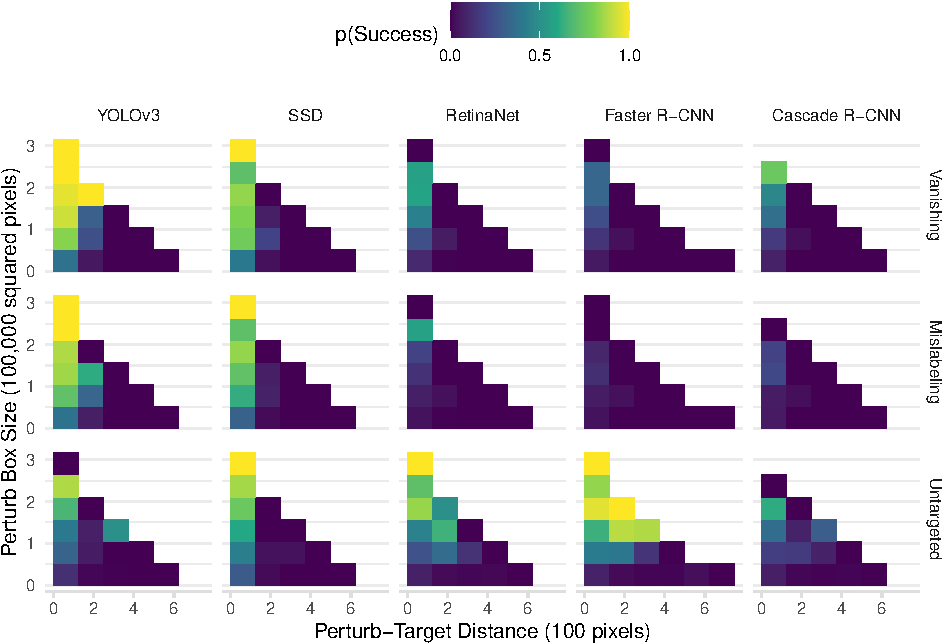
\includegraphics{rmd_imgs/perturb_bbox_and_object_dist_graph-1} 

}

\caption{\textbf{Larger perturb objects significantly increase success rates for all models and attacks, except for mislabeling attack on Faster R-CNN, after controlling for perturb-target distances; Shorter perturb-target distances significantly increase success rates for all models and attacks, after controlling for perturb object sizes:}  The binned summaries graph success proportion against perturb-target distance (100 pixels) and perturb box size (100,000 squared pixels) in the randomized attack experiment.}\label{fig:perturb_bbox_and_object_dist_graph}
\end{figure}

\begingroup\fontsize{9}{11}\selectfont

\begin{longtable}[t]{llllrrrrrr}
\caption{\label{tab:perturb_bbox_and_object_dist_table}We run a logistic model regressing success against perturb-target distance (100 pixels) and perturb box size (100,000 squared pixels) in the randomized attack experiment. Larger perturb objects significantly increase success rates for all models and attacks, except for mislabeling attack on Faster R-CNN, after controlling for perturb-target distances; shorter perturb-target distances significantly increase success rates for all models and attacks, after controlling for perturb object sizes. Table headers are explained in Appendix \ref{app:tab_hdr}.}\\
\toprule
\multicolumn{2}{c}{Group} & \multicolumn{8}{c}{Regression} \\
\cmidrule(l{3pt}r{3pt}){1-2} \cmidrule(l{3pt}r{3pt}){3-10}
 & Attack & term & sig & estimate & std.error & statistic & p.value & conf.low & conf.high\\
\midrule
\addlinespace[0.3em]
\multicolumn{10}{l}{\textbf{YOLOv3}}\\
\hspace{1em} & Vanishing & distance & * & -1.903 & 0.102 & -18.601 & 0.000 & -2.107 & -1.706\\
\cmidrule{3-10}\nopagebreak
\hspace{1em} &  & size & * & 6.436 & 0.407 & 15.804 & 0.000 & 5.656 & 7.252\\
\cmidrule{3-10}\nopagebreak
\hspace{1em} &  & distance * size & * & -2.167 & 0.344 & -6.297 & 0.000 & -2.853 & -1.502\\
\cmidrule{2-10}\nopagebreak
\hspace{1em} & Mislabeling & distance & * & -1.706 & 0.087 & -19.719 & 0.000 & -1.879 & -1.540\\
\cmidrule{3-10}\nopagebreak
\hspace{1em} &  & size & * & 3.182 & 0.270 & 11.791 & 0.000 & 2.667 & 3.724\\
\cmidrule{3-10}\nopagebreak
\hspace{1em} &  & distance * size &  & -0.384 & 0.252 & -1.523 & 0.128 & -0.886 & 0.102\\
\cmidrule{2-10}\nopagebreak
\hspace{1em} & Untargeted & distance & * & -2.191 & 0.160 & -13.656 & 0.000 & -2.515 & -1.886\\
\cmidrule{3-10}\nopagebreak
\hspace{1em} &  & size & * & 1.357 & 0.182 & 7.470 & 0.000 & 1.007 & 1.720\\
\cmidrule{3-10}\nopagebreak
\hspace{1em} &  & distance * size &  & 0.444 & 0.287 & 1.547 & 0.122 & -0.138 & 0.992\\
\cmidrule{1-10}\pagebreak[0]
\addlinespace[0.3em]
\multicolumn{10}{l}{\textbf{SSD}}\\
\hspace{1em} & Vanishing & distance & * & -2.264 & 0.112 & -20.125 & 0.000 & -2.488 & -2.047\\
\cmidrule{3-10}\nopagebreak
\hspace{1em} &  & size & * & 3.896 & 0.313 & 12.467 & 0.000 & 3.299 & 4.524\\
\cmidrule{3-10}\nopagebreak
\hspace{1em} &  & distance * size & * & -0.978 & 0.306 & -3.194 & 0.001 & -1.594 & -0.389\\
\cmidrule{2-10}\nopagebreak
\hspace{1em} & Mislabeling & distance & * & -2.203 & 0.121 & -18.194 & 0.000 & -2.445 & -1.970\\
\cmidrule{3-10}\nopagebreak
\hspace{1em} &  & size & * & 2.787 & 0.252 & 11.061 & 0.000 & 2.306 & 3.295\\
\cmidrule{3-10}\nopagebreak
\hspace{1em} &  & distance * size & * & -0.640 & 0.295 & -2.172 & 0.030 & -1.238 & -0.079\\
\cmidrule{2-10}\nopagebreak
\hspace{1em} & Untargeted & distance & * & -2.299 & 0.124 & -18.514 & 0.000 & -2.547 & -2.060\\
\cmidrule{3-10}\nopagebreak
\hspace{1em} &  & size & * & 1.283 & 0.189 & 6.805 & 0.000 & 0.922 & 1.662\\
\cmidrule{3-10}\nopagebreak
\hspace{1em} &  & distance * size &  & 0.164 & 0.263 & 0.623 & 0.533 & -0.368 & 0.666\\
\cmidrule{1-10}\pagebreak[0]
\addlinespace[0.3em]
\multicolumn{10}{l}{\textbf{RetinaNet}}\\
\hspace{1em} & Vanishing & distance & * & -5.130 & 0.374 & -13.709 & 0.000 & -5.886 & -4.420\\
\cmidrule{3-10}\nopagebreak
\hspace{1em} &  & size & * & 1.912 & 0.249 & 7.695 & 0.000 & 1.440 & 2.415\\
\cmidrule{3-10}\nopagebreak
\hspace{1em} &  & distance * size &  & 0.152 & 0.588 & 0.259 & 0.795 & -1.040 & 1.266\\
\cmidrule{2-10}\nopagebreak
\hspace{1em} & Mislabeling & distance & * & -4.411 & 0.525 & -8.405 & 0.000 & -5.494 & -3.437\\
\cmidrule{3-10}\nopagebreak
\hspace{1em} &  & size & * & 0.920 & 0.248 & 3.703 & 0.000 & 0.435 & 1.410\\
\cmidrule{3-10}\nopagebreak
\hspace{1em} &  & distance * size &  & 0.693 & 0.759 & 0.913 & 0.361 & -0.872 & 2.103\\
\cmidrule{2-10}\nopagebreak
\hspace{1em} & Untargeted & distance & * & -1.555 & 0.151 & -10.285 & 0.000 & -1.862 & -1.270\\
\cmidrule{3-10}\nopagebreak
\hspace{1em} &  & size & * & 1.377 & 0.174 & 7.927 & 0.000 & 1.039 & 1.720\\
\cmidrule{3-10}\nopagebreak
\hspace{1em} &  & distance * size & * & 1.683 & 0.230 & 7.315 & 0.000 & 1.240 & 2.143\\
\cmidrule{1-10}\pagebreak[0]
\addlinespace[0.3em]
\multicolumn{10}{l}{\textbf{Faster R-CNN}}\\
\hspace{1em} & Vanishing & distance & * & -6.113 & 0.604 & -10.114 & 0.000 & -7.351 & -4.982\\
\cmidrule{3-10}\nopagebreak
\hspace{1em} &  & size & * & 1.638 & 0.275 & 5.964 & 0.000 & 1.114 & 2.192\\
\cmidrule{3-10}\nopagebreak
\hspace{1em} &  & distance * size &  & -0.610 & 0.997 & -0.611 & 0.541 & -2.674 & 1.236\\
\cmidrule{2-10}\nopagebreak
\hspace{1em} & Mislabeling & distance & * & -5.569 & 0.630 & -8.839 & 0.000 & -6.870 & -4.398\\
\cmidrule{3-10}\nopagebreak
\hspace{1em} &  & size &  & 0.238 & 0.275 & 0.867 & 0.386 & -0.301 & 0.780\\
\cmidrule{3-10}\nopagebreak
\hspace{1em} &  & distance * size & * & 2.237 & 0.767 & 2.918 & 0.004 & 0.578 & 3.597\\
\cmidrule{2-10}\nopagebreak
\hspace{1em} & Untargeted & distance & * & -1.925 & 0.168 & -11.451 & 0.000 & -2.267 & -1.607\\
\cmidrule{3-10}\nopagebreak
\hspace{1em} &  & size & * & 1.880 & 0.194 & 9.677 & 0.000 & 1.504 & 2.265\\
\cmidrule{3-10}\nopagebreak
\hspace{1em} &  & distance * size & * & 2.143 & 0.259 & 8.262 & 0.000 & 1.648 & 2.665\\
\cmidrule{1-10}\pagebreak[0]
\addlinespace[0.3em]
\multicolumn{10}{l}{\textbf{Cascade R-CNN}}\\
\hspace{1em} & Vanishing & distance & * & -6.971 & 0.573 & -12.163 & 0.000 & -8.137 & -5.890\\
\cmidrule{3-10}\nopagebreak
\hspace{1em} &  & size & * & 2.167 & 0.282 & 7.693 & 0.000 & 1.635 & 2.741\\
\cmidrule{3-10}\nopagebreak
\hspace{1em} &  & distance * size &  & -0.329 & 0.883 & -0.372 & 0.710 & -2.161 & 1.309\\
\cmidrule{2-10}\nopagebreak
\hspace{1em} & Mislabeling & distance & * & -6.440 & 0.585 & -10.999 & 0.000 & -7.639 & -5.343\\
\cmidrule{3-10}\nopagebreak
\hspace{1em} &  & size & * & 0.486 & 0.237 & 2.049 & 0.040 & 0.023 & 0.955\\
\cmidrule{3-10}\nopagebreak
\hspace{1em} &  & distance * size & * & 1.829 & 0.798 & 2.292 & 0.022 & 0.144 & 3.280\\
\cmidrule{2-10}\nopagebreak
\hspace{1em} & Untargeted & distance & * & -2.677 & 0.224 & -11.971 & 0.000 & -3.132 & -2.255\\
\cmidrule{3-10}\nopagebreak
\hspace{1em} &  & size & * & 0.693 & 0.174 & 3.991 & 0.000 & 0.352 & 1.034\\
\cmidrule{3-10}\nopagebreak
\hspace{1em} &  & distance * size & * & 2.181 & 0.258 & 8.442 & 0.000 & 1.678 & 2.693\\
\bottomrule
\end{longtable}
\endgroup{}

\begin{figure}[tb]

{\centering 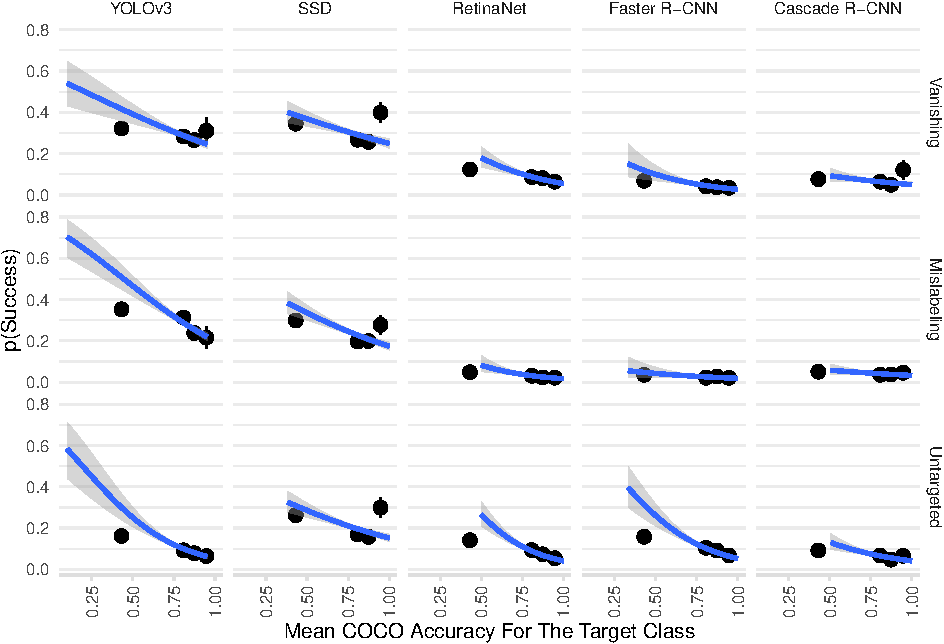
\includegraphics{rmd_imgs/target_success_graph-1} 

}

\caption{\textbf{Although higher mean COCO accuracy for the target class seem to decrease success rates, the results are mixed after controlling for target class confidence (Table \ref{tab:target_success_table}):}  The binned summaries and regression trendlines graph success proportion against mean COCO accuracy for the target class in the randomized attack experiment. Bins are split into quantiles. Errors are 95\% confidence intervals. }\label{fig:target_success_graph}
\end{figure}

\begingroup\fontsize{9}{11}\selectfont

\begin{longtable}[t]{llllrrrrrr}
\caption{\label{tab:target_success_table}We run a logistic model regressing success against mean COCO accuracy for the target class, with target confidence as covariate, in the randomized attack experiment. The results are mixed after controlling for target class confidence and the relatively large interaction terms make interpretation challenging. Table headers are explained in Appendix \ref{app:tab_hdr}.}\\
\toprule
\multicolumn{2}{c}{Group} & \multicolumn{8}{c}{Regression} \\
\cmidrule(l{3pt}r{3pt}){1-2} \cmidrule(l{3pt}r{3pt}){3-10}
 & Attack & term & sig & estimate & std.error & statistic & p.value & conf.low & conf.high\\
\midrule
\addlinespace[0.3em]
\multicolumn{10}{l}{\textbf{YOLOv3}}\\
\hspace{1em} & Vanishing & accuracy &  & -0.436 & 1.053 & -0.414 & 0.679 & -2.497 & 1.634\\
\cmidrule{3-10}\nopagebreak
\hspace{1em} &  & confidence &  & 0.475 & 1.145 & 0.415 & 0.678 & -1.771 & 2.722\\
\cmidrule{3-10}\nopagebreak
\hspace{1em} &  & accuracy * confidence &  & -1.233 & 1.414 & -0.873 & 0.383 & -4.007 & 1.538\\
\cmidrule{2-10}\nopagebreak
\hspace{1em} & Mislabeling & accuracy &  & 0.159 & 1.034 & 0.154 & 0.877 & -1.871 & 2.186\\
\cmidrule{3-10}\nopagebreak
\hspace{1em} &  & confidence &  & 0.538 & 1.147 & 0.469 & 0.639 & -1.716 & 2.782\\
\cmidrule{3-10}\nopagebreak
\hspace{1em} &  & accuracy * confidence & * & -2.902 & 1.418 & -2.047 & 0.041 & -5.679 & -0.118\\
\cmidrule{2-10}\nopagebreak
\hspace{1em} & Untargeted & accuracy & * & -3.282 & 1.330 & -2.468 & 0.014 & -5.906 & -0.689\\
\cmidrule{3-10}\nopagebreak
\hspace{1em} &  & confidence & * & -4.205 & 1.659 & -2.535 & 0.011 & -7.517 & -1.009\\
\cmidrule{3-10}\nopagebreak
\hspace{1em} &  & accuracy * confidence &  & 1.199 & 2.069 & 0.580 & 0.562 & -2.799 & 5.314\\
\cmidrule{1-10}\pagebreak[0]
\addlinespace[0.3em]
\multicolumn{10}{l}{\textbf{SSD}}\\
\hspace{1em} & Vanishing & accuracy &  & -0.743 & 0.817 & -0.909 & 0.363 & -2.342 & 0.864\\
\cmidrule{3-10}\nopagebreak
\hspace{1em} &  & confidence &  & -0.042 & 0.869 & -0.048 & 0.962 & -1.746 & 1.664\\
\cmidrule{3-10}\nopagebreak
\hspace{1em} &  & accuracy * confidence &  & -0.396 & 1.089 & -0.363 & 0.716 & -2.532 & 1.740\\
\cmidrule{2-10}\nopagebreak
\hspace{1em} & Mislabeling & accuracy &  & -0.797 & 0.842 & -0.946 & 0.344 & -2.444 & 0.857\\
\cmidrule{3-10}\nopagebreak
\hspace{1em} &  & confidence &  & -0.277 & 0.910 & -0.305 & 0.761 & -2.064 & 1.504\\
\cmidrule{3-10}\nopagebreak
\hspace{1em} &  & accuracy * confidence &  & -0.977 & 1.145 & -0.853 & 0.394 & -3.221 & 1.271\\
\cmidrule{2-10}\nopagebreak
\hspace{1em} & Untargeted & accuracy & * & -2.087 & 0.867 & -2.408 & 0.016 & -3.789 & -0.389\\
\cmidrule{3-10}\nopagebreak
\hspace{1em} &  & confidence & * & -3.125 & 0.990 & -3.157 & 0.002 & -5.081 & -1.198\\
\cmidrule{3-10}\nopagebreak
\hspace{1em} &  & accuracy * confidence &  & 1.486 & 1.241 & 1.198 & 0.231 & -0.933 & 3.932\\
\cmidrule{1-10}\pagebreak[0]
\addlinespace[0.3em]
\multicolumn{10}{l}{\textbf{RetinaNet}}\\
\hspace{1em} & Vanishing & accuracy & * & -3.520 & 1.630 & -2.160 & 0.031 & -6.700 & -0.309\\
\cmidrule{3-10}\nopagebreak
\hspace{1em} &  & confidence & * & -6.644 & 2.646 & -2.511 & 0.012 & -11.879 & -1.504\\
\cmidrule{3-10}\nopagebreak
\hspace{1em} &  & accuracy * confidence &  & 4.770 & 3.090 & 1.544 & 0.123 & -1.259 & 10.858\\
\cmidrule{2-10}\nopagebreak
\hspace{1em} & Mislabeling & accuracy & * & -7.902 & 2.929 & -2.697 & 0.007 & -13.606 & -2.128\\
\cmidrule{3-10}\nopagebreak
\hspace{1em} &  & confidence & * & -20.491 & 5.908 & -3.469 & 0.001 & -32.313 & -9.179\\
\cmidrule{3-10}\nopagebreak
\hspace{1em} &  & accuracy * confidence & * & 17.153 & 6.788 & 2.527 & 0.012 & 4.011 & 30.592\\
\cmidrule{2-10}\nopagebreak
\hspace{1em} & Untargeted & accuracy & * & -4.352 & 1.707 & -2.549 & 0.011 & -7.701 & -1.007\\
\cmidrule{3-10}\nopagebreak
\hspace{1em} &  & confidence & * & -9.046 & 2.985 & -3.030 & 0.002 & -14.984 & -3.279\\
\cmidrule{3-10}\nopagebreak
\hspace{1em} &  & accuracy * confidence &  & 5.142 & 3.520 & 1.461 & 0.144 & -1.699 & 12.099\\
\cmidrule{1-10}\pagebreak[0]
\addlinespace[0.3em]
\multicolumn{10}{l}{\textbf{Faster R-CNN}}\\
\hspace{1em} & Vanishing & accuracy & * & 4.935 & 2.132 & 2.315 & 0.021 & 0.839 & 9.204\\
\cmidrule{3-10}\nopagebreak
\hspace{1em} &  & confidence & * & 4.666 & 2.288 & 2.040 & 0.041 & 0.200 & 9.180\\
\cmidrule{3-10}\nopagebreak
\hspace{1em} &  & accuracy * confidence & * & -9.142 & 2.824 & -3.238 & 0.001 & -14.707 & -3.627\\
\cmidrule{2-10}\nopagebreak
\hspace{1em} & Mislabeling & accuracy & * & 8.515 & 2.767 & 3.078 & 0.002 & 3.222 & 14.084\\
\cmidrule{3-10}\nopagebreak
\hspace{1em} &  & confidence & * & 6.412 & 3.183 & 2.015 & 0.044 & 0.114 & 12.625\\
\cmidrule{3-10}\nopagebreak
\hspace{1em} &  & accuracy * confidence & * & -12.713 & 3.888 & -3.270 & 0.001 & -20.304 & -5.038\\
\cmidrule{2-10}\nopagebreak
\hspace{1em} & Untargeted & accuracy &  & 1.447 & 1.442 & 1.003 & 0.316 & -1.373 & 4.289\\
\cmidrule{3-10}\nopagebreak
\hspace{1em} &  & confidence &  & 0.733 & 1.588 & 0.462 & 0.644 & -2.395 & 3.836\\
\cmidrule{3-10}\nopagebreak
\hspace{1em} &  & accuracy * confidence & * & -5.146 & 1.969 & -2.614 & 0.009 & -8.999 & -1.273\\
\cmidrule{1-10}\pagebreak[0]
\addlinespace[0.3em]
\multicolumn{10}{l}{\textbf{Cascade R-CNN}}\\
\hspace{1em} & Vanishing & accuracy &  & 1.644 & 2.104 & 0.781 & 0.435 & -2.419 & 5.840\\
\cmidrule{3-10}\nopagebreak
\hspace{1em} &  & confidence &  & 0.766 & 2.173 & 0.353 & 0.724 & -3.466 & 5.064\\
\cmidrule{3-10}\nopagebreak
\hspace{1em} &  & accuracy * confidence &  & -2.987 & 2.679 & -1.115 & 0.265 & -8.273 & 2.237\\
\cmidrule{2-10}\nopagebreak
\hspace{1em} & Mislabeling & accuracy & * & 4.762 & 2.347 & 2.029 & 0.042 & 0.236 & 9.446\\
\cmidrule{3-10}\nopagebreak
\hspace{1em} &  & confidence &  & 1.915 & 2.651 & 0.722 & 0.470 & -3.301 & 7.107\\
\cmidrule{3-10}\nopagebreak
\hspace{1em} &  & accuracy * confidence & * & -6.491 & 3.243 & -2.002 & 0.045 & -12.843 & -0.119\\
\cmidrule{2-10}\nopagebreak
\hspace{1em} & Untargeted & accuracy & * & 3.752 & 1.805 & 2.079 & 0.038 & 0.241 & 7.324\\
\cmidrule{3-10}\nopagebreak
\hspace{1em} &  & confidence &  & 1.669 & 2.033 & 0.821 & 0.412 & -2.339 & 5.637\\
\cmidrule{3-10}\nopagebreak
\hspace{1em} &  & accuracy * confidence & * & -6.887 & 2.519 & -2.734 & 0.006 & -11.812 & -1.930\\
\bottomrule
\end{longtable}
\endgroup{}

\begin{figure}[tb]

{\centering 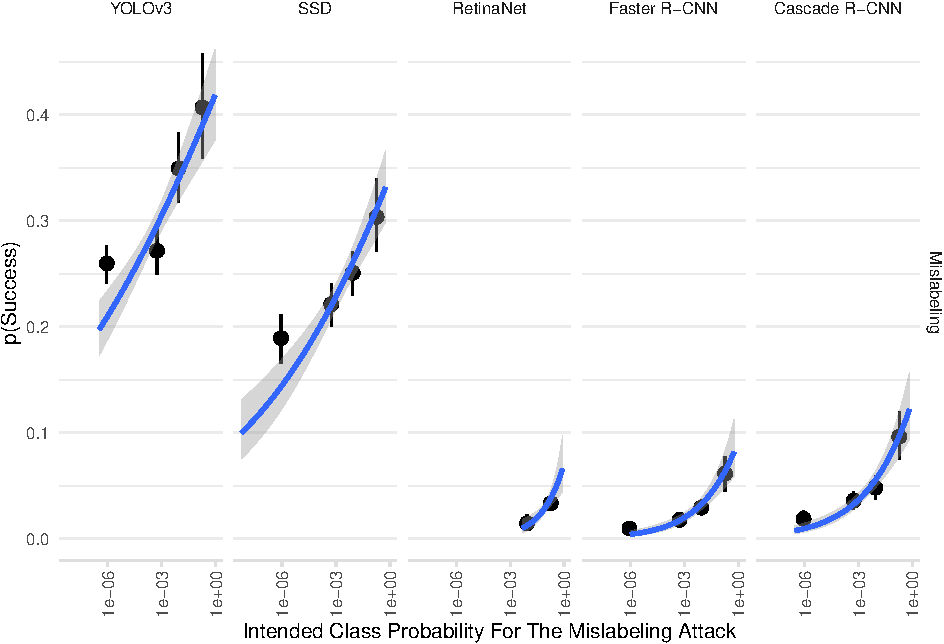
\includegraphics{rmd_imgs/mislabel_conf_graph-1} 

}

\caption{\textbf{Although intended class probability seem to increase success rates for the mislabeling attack, it does not predict success rates after controlling for target class confidence, except for RetinaNet (Table \ref{tab:mislabel_conf_table}):}  The binned summaries and regression trendlines graph success proportion against intended class probability in the randomized attack experiment. Bins are split into quantiles. Errors are 95\% confidence intervals. }\label{fig:mislabel_conf_graph}
\end{figure}

\begingroup\fontsize{9}{11}\selectfont

\begin{longtable}[t]{llllrrrrrr}
\caption{\label{tab:mislabel_conf_table}We run a logistic model regressing success against log(intended class probability) for the mislabeling attack, with predicted class's confidence as covariate, in the randomized attack experiment. Intended class probability does not predict success rates after controlling for target class confidence, except for RetinaNet. Table headers are explained in Appendix \ref{app:tab_hdr}.}\\
\toprule
\multicolumn{2}{c}{Group} & \multicolumn{8}{c}{Regression} \\
\cmidrule(l{3pt}r{3pt}){1-2} \cmidrule(l{3pt}r{3pt}){3-10}
 & Model & term & sig & estimate & std.error & statistic & p.value & conf.low & conf.high\\
\midrule
\addlinespace[0.3em]
\multicolumn{10}{l}{\textbf{Mislabeling}}\\
\hspace{1em} & YOLOv3 & log(probability) &  & 0.052 & 0.036 & 1.425 & 0.154 & -0.019 & 0.123\\
\cmidrule{3-10}\nopagebreak
\hspace{1em} &  & confidence & * & -1.777 & 0.431 & -4.125 & 0.000 & -2.624 & -0.935\\
\cmidrule{3-10}\nopagebreak
\hspace{1em} &  & log(probability) * confidence &  & 0.010 & 0.050 & 0.193 & 0.847 & -0.089 & 0.108\\
\cmidrule{2-10}\nopagebreak
\hspace{1em} & SSD & log(probability) &  & 0.034 & 0.042 & 0.791 & 0.429 & -0.049 & 0.117\\
\cmidrule{3-10}\nopagebreak
\hspace{1em} &  & confidence & * & -0.760 & 0.375 & -2.026 & 0.043 & -1.494 & -0.023\\
\cmidrule{3-10}\nopagebreak
\hspace{1em} &  & log(probability) * confidence &  & 0.025 & 0.054 & 0.473 & 0.636 & -0.080 & 0.131\\
\cmidrule{2-10}\nopagebreak
\hspace{1em} & RetinaNet & log(probability) & * & 0.626 & 0.310 & 2.018 & 0.044 & 0.003 & 1.218\\
\cmidrule{3-10}\nopagebreak
\hspace{1em} &  & confidence & * & -8.462 & 1.804 & -4.691 & 0.000 & -12.016 & -4.950\\
\cmidrule{3-10}\nopagebreak
\hspace{1em} &  & log(probability) * confidence &  & -1.016 & 0.648 & -1.568 & 0.117 & -2.242 & 0.295\\
\cmidrule{2-10}\nopagebreak
\hspace{1em} & Faster R-CNN & log(probability) &  & 0.060 & 0.100 & 0.593 & 0.553 & -0.137 & 0.257\\
\cmidrule{3-10}\nopagebreak
\hspace{1em} &  & confidence & * & -3.022 & 0.925 & -3.265 & 0.001 & -4.835 & -1.201\\
\cmidrule{3-10}\nopagebreak
\hspace{1em} &  & log(probability) * confidence &  & 0.076 & 0.147 & 0.521 & 0.603 & -0.207 & 0.368\\
\cmidrule{2-10}\nopagebreak
\hspace{1em} & Cascade R-CNN & log(probability) &  & 0.117 & 0.080 & 1.474 & 0.140 & -0.039 & 0.274\\
\cmidrule{3-10}\nopagebreak
\hspace{1em} &  & confidence & * & -2.872 & 0.722 & -3.979 & 0.000 & -4.283 & -1.450\\
\cmidrule{3-10}\nopagebreak
\hspace{1em} &  & log(probability) * confidence &  & -0.014 & 0.108 & -0.130 & 0.897 & -0.224 & 0.200\\
\bottomrule
\end{longtable}
\endgroup{}

\begin{figure}[tb]

{\centering 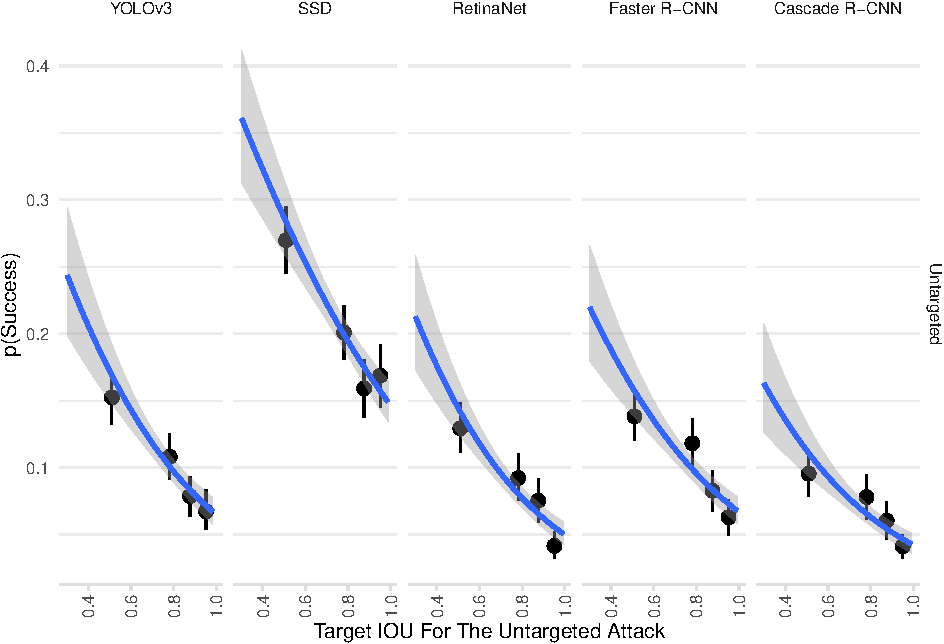
\includegraphics{rmd_imgs/untarget_iou_graph-1} 

}

\caption{\textbf{Target IOU for the untargeted attack increases success rates on all models:}  The binned summaries and regression trendlines graph success proportion against target IOU for the untargeted attack in the randomized attack experiment. Bins are split into quantiles. Errors are 95\% confidence intervals. }\label{fig:untarget_iou_graph}
\end{figure}

\begingroup\fontsize{9}{11}\selectfont

\begin{longtable}[t]{llllrrrrrr}
\caption{\label{tab:untarget_iou_table}We run a logistic model regressing success against target IOU for the untargeted attack in the randomized attack experiment. Target IOU for the untargeted attack increases success rates on all models. Table headers are explained in Appendix \ref{app:tab_hdr}.}\\
\toprule
\multicolumn{2}{c}{Group} & \multicolumn{8}{c}{Regression} \\
\cmidrule(l{3pt}r{3pt}){1-2} \cmidrule(l{3pt}r{3pt}){3-10}
 & Model & term & sig & estimate & std.error & statistic & p.value & conf.low & conf.high\\
\midrule
\addlinespace[0.3em]
\multicolumn{10}{l}{\textbf{Untargeted}}\\
\hspace{1em} & YOLOv3 & iou & * & -2.199 & 0.278 & -7.904 & 0 & -2.741 & -1.650\\
\cmidrule{2-10}\nopagebreak
\hspace{1em} & SSD & iou & * & -1.704 & 0.226 & -7.549 & 0 & -2.146 & -1.260\\
\cmidrule{2-10}\nopagebreak
\hspace{1em} & RetinaNet & iou & * & -2.344 & 0.275 & -8.533 & 0 & -2.880 & -1.802\\
\cmidrule{2-10}\nopagebreak
\hspace{1em} & Faster R-CNN & iou & * & -1.961 & 0.267 & -7.340 & 0 & -2.481 & -1.433\\
\cmidrule{2-10}\nopagebreak
\hspace{1em} & Cascade R-CNN & iou & * & -2.122 & 0.307 & -6.902 & 0 & -2.718 & -1.512\\
\bottomrule
\end{longtable}
\endgroup{}
